\documentclass{standalone}
\usepackage{tikz}
\usetikzlibrary{patterns, positioning}
\usepackage[sfdefault]{ClearSans} %% option 'sfdefault' activates Clear Sans as the default text font
\usepackage[T1]{fontenc}

\begin{document}
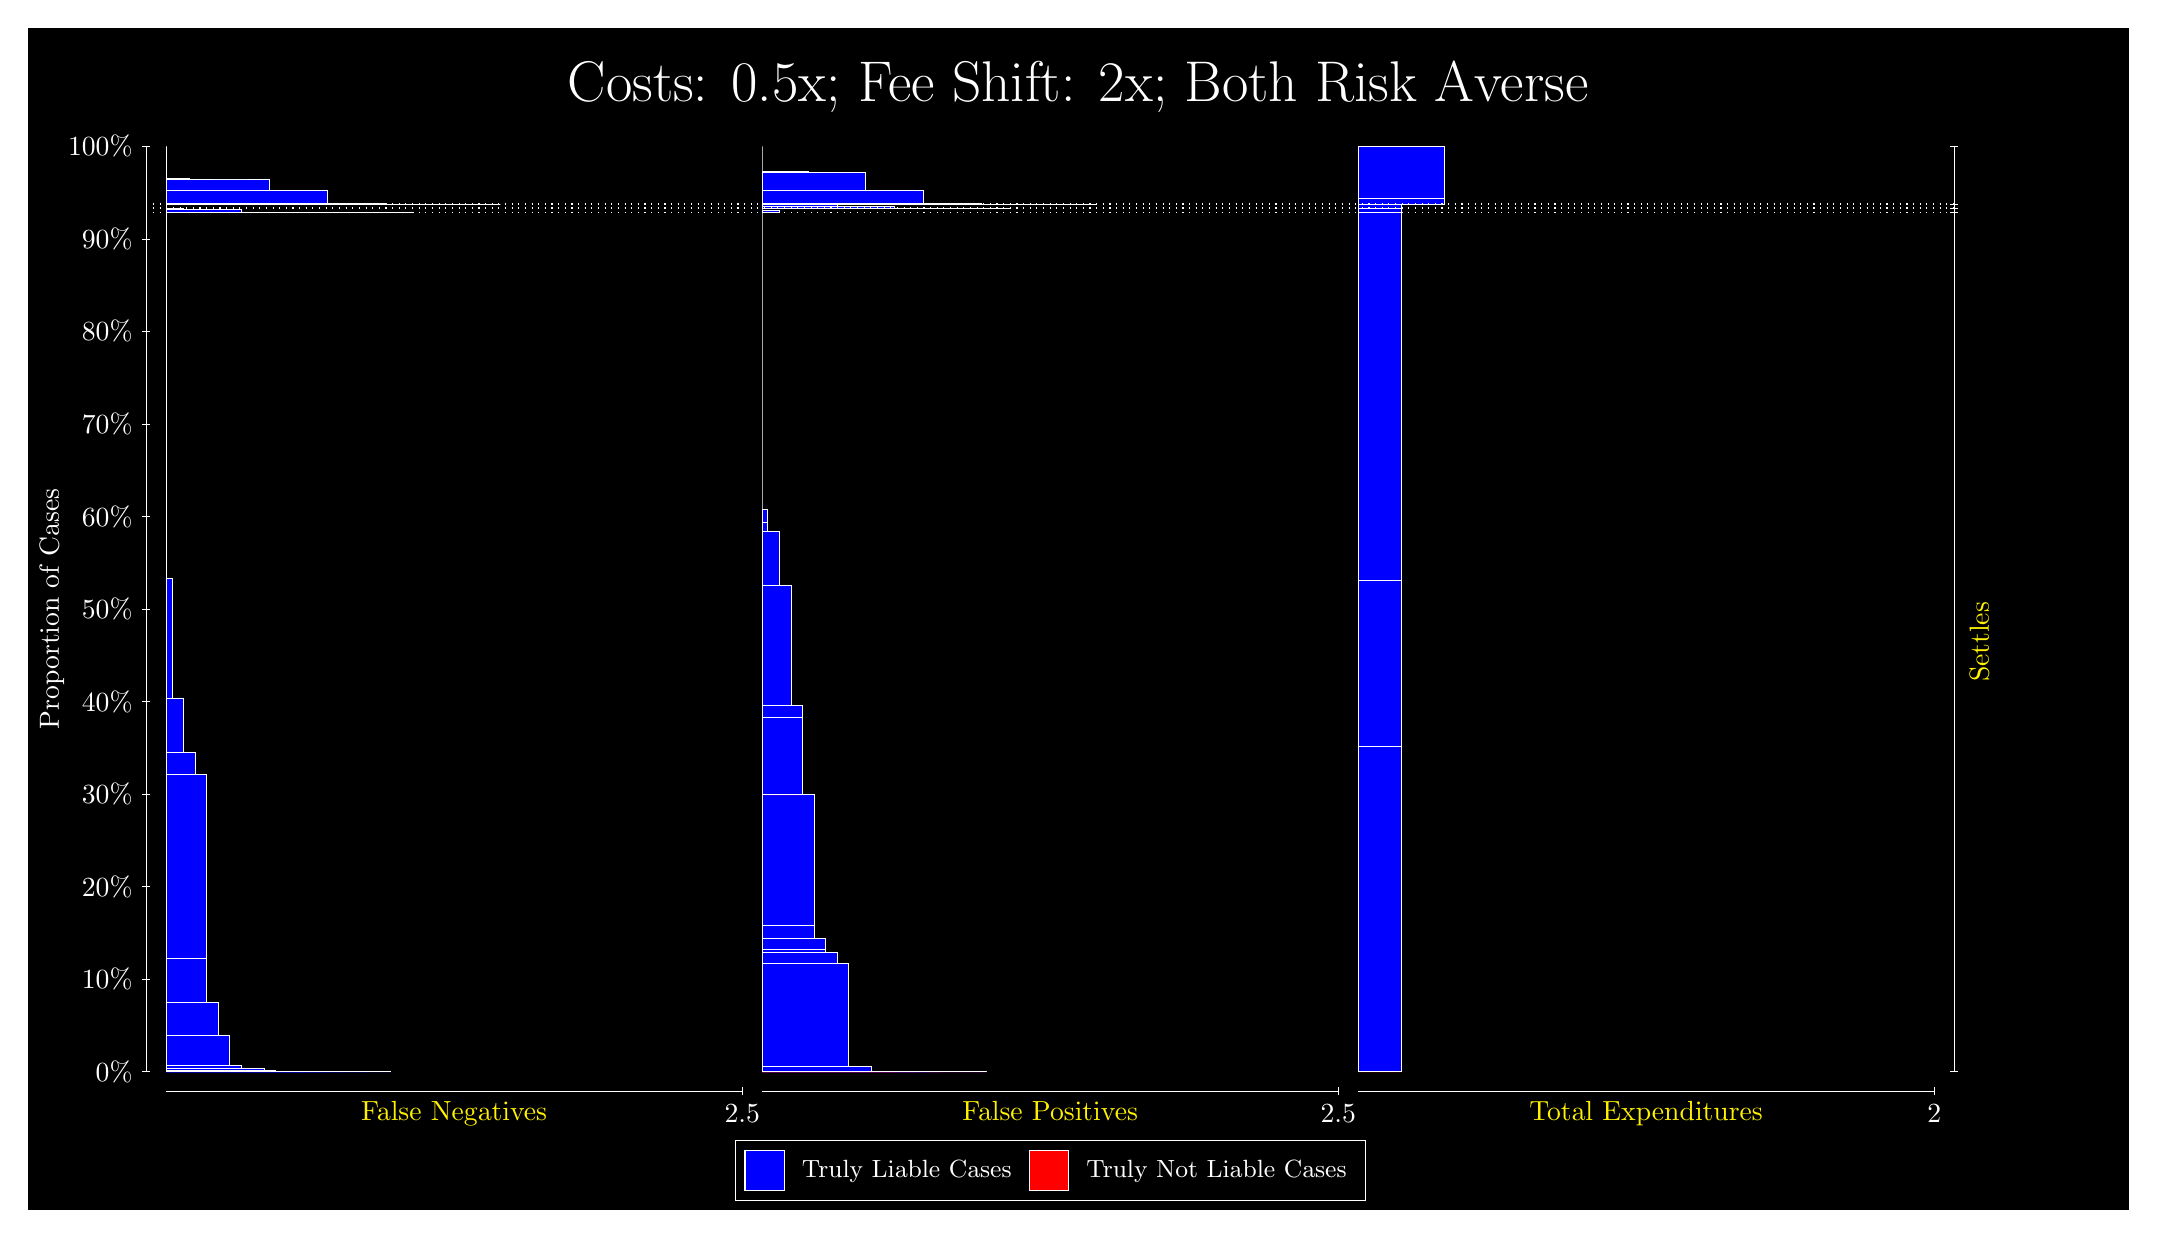
\begin{tikzpicture}
\draw[fill=black] (0,0) rectangle (26.667,15);
\draw[text=white] (0,13.5) rectangle (26.667,15) node[midway] {\huge Costs: 0.5x; Fee Shift: 2x; Both Risk Averse};
\draw[white, very thin] (1.5,1.75) -- (1.5,13.5);
\node[rotate=90, text=white, anchor=center] at (0.3, 7.625) {Proportion of Cases};
\draw[white, very thin] (1.45,1.75) -- (1.55,1.75);
\node[text=white, anchor=east] at (1.45, 1.75) {0\%};
\draw[white, very thin] (1.45,2.925) -- (1.55,2.925);
\node[text=white, anchor=east] at (1.45, 2.925) {10\%};
\draw[white, very thin] (1.45,4.1) -- (1.55,4.1);
\node[text=white, anchor=east] at (1.45, 4.1) {20\%};
\draw[white, very thin] (1.45,5.275) -- (1.55,5.275);
\node[text=white, anchor=east] at (1.45, 5.275) {30\%};
\draw[white, very thin] (1.45,6.45) -- (1.55,6.45);
\node[text=white, anchor=east] at (1.45, 6.45) {40\%};
\draw[white, very thin] (1.45,7.625) -- (1.55,7.625);
\node[text=white, anchor=east] at (1.45, 7.625) {50\%};
\draw[white, very thin] (1.45,8.8) -- (1.55,8.8);
\node[text=white, anchor=east] at (1.45, 8.8) {60\%};
\draw[white, very thin] (1.45,9.975) -- (1.55,9.975);
\node[text=white, anchor=east] at (1.45, 9.975) {70\%};
\draw[white, very thin] (1.45,11.15) -- (1.55,11.15);
\node[text=white, anchor=east] at (1.45, 11.15) {80\%};
\draw[white, very thin] (1.45,12.325) -- (1.55,12.325);
\node[text=white, anchor=east] at (1.45, 12.325) {90\%};
\draw[white, very thin] (1.45,13.5) -- (1.55,13.5);
\node[text=white, anchor=east] at (1.45, 13.5) {100\%};

\draw[white, very thin] (24.457,1.75) -- (24.457,13.5);
\draw[white, very thin] (24.407,1.75) -- (24.507,1.75);
\node[anchor=west] at (24.407, 1.75) {};
\draw[white, very thin] (24.407,12.664) -- (24.507,12.664);
\node[anchor=west] at (24.407, 12.664) {};
\draw[white, very thin] (24.407,12.717) -- (24.507,12.717);
\node[anchor=west] at (24.407, 12.717) {};
\draw[white, very thin] (24.407,12.767) -- (24.507,12.767);
\node[anchor=west] at (24.407, 12.767) {};
\draw[white, very thin] (24.407,13.5) -- (24.507,13.5);
\node[anchor=west] at (24.407, 13.5) {};

\draw[white, very thin, fill=blue] (1.75,1.75) rectangle (4.6044,1.75);
\draw[white, very thin, fill=blue] (1.75,1.75) rectangle (4.3116,1.75);
\draw[white, very thin, fill=blue] (1.75,1.75) rectangle (4.0188,1.75);
\draw[white, very thin, fill=blue] (1.75,1.75) rectangle (3.8725,1.75);
\draw[white, very thin, fill=blue] (1.75,1.75) rectangle (3.7261,1.75);
\draw[white, very thin, fill=blue] (1.75,1.75) rectangle (3.5797,1.75);
\draw[white, very thin, fill=blue] (1.75,1.75) rectangle (3.4333,1.75);
\draw[white, very thin, fill=blue] (1.75,1.75) rectangle (3.287,1.7551);
\draw[white, very thin, fill=blue] (1.75,1.7551) rectangle (3.1406,1.7626);
\draw[white, very thin, fill=blue] (1.75,1.7626) rectangle (2.9942,1.7862);
\draw[white, very thin, fill=blue] (1.75,1.7862) rectangle (2.8478,1.7931);
\draw[white, very thin, fill=blue] (1.75,1.7931) rectangle (2.7015,1.8247);
\draw[white, very thin, fill=blue] (1.75,1.8247) rectangle (2.5551,2.2127);
\draw[white, very thin, fill=blue] (1.75,2.2127) rectangle (2.4087,2.6354);
\draw[white, very thin, fill=blue] (1.75,2.6354) rectangle (2.2623,3.1846);
\draw[white, very thin, fill=blue] (1.75,3.1846) rectangle (2.2623,5.527);
\draw[white, very thin, fill=blue] (1.75,5.527) rectangle (2.1159,5.8066);
\draw[white, very thin, fill=blue] (1.75,5.8066) rectangle (1.9696,6.4874);
\draw[white, very thin, fill=blue] (1.75,6.4874) rectangle (1.8232,8.0172);
\draw[white, very thin, fill=red] (1.75,8.0172) rectangle (1.75,8.0172);
\draw[white, very thin, fill=blue] (1.75,8.0172) rectangle (1.75,12.664);
\draw[white, very thin, fill=blue] (1.75,12.664) rectangle (4.8971,12.664);
\draw[white, very thin, fill=blue] (1.75,12.664) rectangle (4.1652,12.664);
\draw[white, very thin, fill=blue] (1.75,12.664) rectangle (3.4333,12.665);
\draw[white, very thin, fill=blue] (1.75,12.665) rectangle (2.7015,12.697);
\draw[white, very thin, fill=blue] (1.75,12.697) rectangle (1.9696,12.717);
\draw[white, very thin, fill=red] (1.75,12.717) rectangle (1.75,12.717);
\draw[white, very thin, fill=blue] (1.75,12.717) rectangle (1.9696,12.717);
\draw[white, very thin, fill=red] (1.75,12.717) rectangle (1.75,12.717);
\draw[white, very thin, fill=blue] (1.75,12.717) rectangle (1.75,12.767);
\draw[white, very thin, fill=blue] (1.75,12.767) rectangle (5.9949,12.767);
\draw[white, very thin, fill=blue] (1.75,12.767) rectangle (5.2631,12.767);
\draw[white, very thin, fill=blue] (1.75,12.767) rectangle (4.5312,12.782);
\draw[white, very thin, fill=blue] (1.75,12.782) rectangle (3.7993,12.943);
\draw[white, very thin, fill=blue] (1.75,12.943) rectangle (3.5065,12.943);
\draw[white, very thin, fill=blue] (1.75,12.943) rectangle (3.0674,13.085);
\draw[white, very thin, fill=blue] (1.75,13.085) rectangle (2.7746,13.085);
\draw[white, very thin, fill=blue] (1.75,13.085) rectangle (2.3355,13.086);
\draw[white, very thin, fill=blue] (1.75,13.086) rectangle (2.0428,13.095);
\draw[white, very thin, fill=red] (1.75,13.095) rectangle (1.75,13.095);
\draw[white, very thin, fill=blue] (1.75,13.095) rectangle (1.75,13.5);
\draw[white, very thin, fill=red] (9.3189,1.75) rectangle (12.173,1.75);
\draw[white, very thin, fill=blue] (9.3189,1.75) rectangle (12.173,1.75);
\draw[white, very thin, fill=red] (9.3189,1.75) rectangle (11.588,1.75);
\draw[white, very thin, fill=blue] (9.3189,1.75) rectangle (11.588,1.75);
\draw[white, very thin, fill=blue] (9.3189,1.75) rectangle (11.441,1.75);
\draw[white, very thin, fill=red] (9.3189,1.75) rectangle (11.295,1.75);
\draw[white, very thin, fill=blue] (9.3189,1.75) rectangle (11.295,1.75);
\draw[white, very thin, fill=red] (9.3189,1.75) rectangle (11.002,1.75);
\draw[white, very thin, fill=blue] (9.3189,1.75) rectangle (11.002,1.7521);
\draw[white, very thin, fill=blue] (9.3189,1.7521) rectangle (10.856,1.7525);
\draw[white, very thin, fill=red] (9.3189,1.7525) rectangle (10.709,1.7525);
\draw[white, very thin, fill=blue] (9.3189,1.7525) rectangle (10.709,1.7547);
\draw[white, very thin, fill=blue] (9.3189,1.7547) rectangle (10.709,1.8138);
\draw[white, very thin, fill=blue] (9.3189,1.8138) rectangle (10.563,1.8154);
\draw[white, very thin, fill=red] (9.3189,1.8154) rectangle (10.417,1.8154);
\draw[white, very thin, fill=blue] (9.3189,1.8154) rectangle (10.417,3.1205);
\draw[white, very thin, fill=blue] (9.3189,3.1205) rectangle (10.27,3.2633);
\draw[white, very thin, fill=red] (9.3189,3.2633) rectangle (10.124,3.2633);
\draw[white, very thin, fill=blue] (9.3189,3.2633) rectangle (10.124,3.304);
\draw[white, very thin, fill=blue] (9.3189,3.304) rectangle (10.124,3.4389);
\draw[white, very thin, fill=blue] (9.3189,3.4389) rectangle (9.9776,3.6034);
\draw[white, very thin, fill=blue] (9.3189,3.6034) rectangle (9.9776,5.2661);
\draw[white, very thin, fill=red] (9.3189,5.2661) rectangle (9.8312,5.2661);
\draw[white, very thin, fill=blue] (9.3189,5.2661) rectangle (9.8312,6.2449);
\draw[white, very thin, fill=blue] (9.3189,6.2449) rectangle (9.8312,6.397);
\draw[white, very thin, fill=blue] (9.3189,6.397) rectangle (9.6848,7.9269);
\draw[white, very thin, fill=blue] (9.3189,7.9269) rectangle (9.5384,8.6077);
\draw[white, very thin, fill=blue] (9.3189,8.6077) rectangle (9.3921,8.7249);
\draw[white, very thin, fill=blue] (9.3189,8.7249) rectangle (9.3921,8.8873);
\draw[white, very thin, fill=blue] (9.3189,8.8873) rectangle (9.3189,12.664);
\draw[white, very thin, fill=red] (9.3189,12.664) rectangle (9.5384,12.664);
\draw[white, very thin, fill=blue] (9.3189,12.664) rectangle (9.5384,12.684);
\draw[white, very thin, fill=blue] (9.3189,12.684) rectangle (9.3189,12.717);
\draw[white, very thin, fill=red] (9.3189,12.717) rectangle (12.466,12.717);
\draw[white, very thin, fill=blue] (9.3189,12.717) rectangle (12.466,12.717);
\draw[white, very thin, fill=blue] (9.3189,12.717) rectangle (11.734,12.717);
\draw[white, very thin, fill=blue] (9.3189,12.717) rectangle (11.002,12.741);
\draw[white, very thin, fill=blue] (9.3189,12.741) rectangle (10.27,12.767);
\draw[white, very thin, fill=blue] (9.3189,12.767) rectangle (9.5384,12.767);
\draw[white, very thin, fill=red] (9.3189,12.767) rectangle (13.564,12.767);
\draw[white, very thin, fill=blue] (9.3189,12.767) rectangle (13.564,12.767);
\draw[white, very thin, fill=red] (9.3189,12.767) rectangle (12.832,12.767);
\draw[white, very thin, fill=blue] (9.3189,12.767) rectangle (12.832,12.767);
\draw[white, very thin, fill=red] (9.3189,12.767) rectangle (12.1,12.767);
\draw[white, very thin, fill=blue] (9.3189,12.767) rectangle (12.1,12.777);
\draw[white, very thin, fill=red] (9.3189,12.777) rectangle (11.368,12.777);
\draw[white, very thin, fill=blue] (9.3189,12.777) rectangle (11.368,12.947);
\draw[white, very thin, fill=blue] (9.3189,12.947) rectangle (10.636,13.172);
\draw[white, very thin, fill=red] (9.3189,13.172) rectangle (10.344,13.172);
\draw[white, very thin, fill=blue] (9.3189,13.172) rectangle (10.344,13.172);
\draw[white, very thin, fill=blue] (9.3189,13.172) rectangle (9.9044,13.181);
\draw[white, very thin, fill=red] (9.3189,13.181) rectangle (9.6116,13.181);
\draw[white, very thin, fill=blue] (9.3189,13.181) rectangle (9.6116,13.181);
\draw[white, very thin, fill=blue] (9.3189,13.181) rectangle (9.6116,13.182);
\draw[white, very thin, fill=red] (9.3189,13.182) rectangle (9.3189,13.182);
\draw[white, very thin, fill=blue] (9.3189,13.182) rectangle (9.3189,13.5);
\draw[white, very thin, fill=red] (16.888,1.75) rectangle (17.437,1.75);
\draw[white, very thin, fill=blue] (16.888,1.75) rectangle (17.437,5.8804);
\draw[white, very thin, fill=red] (16.888,5.8804) rectangle (17.437,5.8804);
\draw[white, very thin, fill=blue] (16.888,5.8804) rectangle (17.437,7.9945);
\draw[white, very thin, fill=red] (16.888,7.9945) rectangle (17.437,7.9945);
\draw[white, very thin, fill=blue] (16.888,7.9945) rectangle (17.437,12.664);
\draw[white, very thin, fill=red] (16.888,12.664) rectangle (17.437,12.664);
\draw[white, very thin, fill=blue] (16.888,12.664) rectangle (17.437,12.717);
\draw[white, very thin, fill=red] (16.888,12.717) rectangle (17.437,12.717);
\draw[white, very thin, fill=blue] (16.888,12.717) rectangle (17.437,12.767);
\draw[white, very thin, fill=red] (16.888,12.767) rectangle (17.986,12.767);
\draw[white, very thin, fill=blue] (16.888,12.767) rectangle (17.986,12.845);
\draw[white, very thin, fill=red] (16.888,12.845) rectangle (17.986,12.845);
\draw[white, very thin, fill=blue] (16.888,12.845) rectangle (17.986,13.5);
\draw[white, dotted] (1.5,12.664) -- (24.457,12.664);
\draw[white, dotted] (1.5,12.717) -- (24.457,12.717);
\draw[white, dotted] (1.5,12.767) -- (24.457,12.767);
\draw[white, very thin] (1.75,1.5) -- (9.0689,1.5);
\node[text=yellow, anchor=north] at (5.4094, 1.5) {False Negatives};
\draw[white, very thin] (9.0689,1.45) -- (9.0689,1.55);
\node[text=white, anchor=north] at (9.0689, 1.45) {2.5};

\draw[white, very thin] (9.3189,1.5) -- (16.638,1.5);
\node[text=yellow, anchor=north] at (12.978, 1.5) {False Positives};
\draw[white, very thin] (16.638,1.45) -- (16.638,1.55);
\node[text=white, anchor=north] at (16.638, 1.45) {2.5};

\draw[white, very thin] (16.888,1.5) -- (24.207,1.5);
\node[text=yellow, anchor=north] at (20.547, 1.5) {Total Expenditures};
\draw[white, very thin] (24.207,1.45) -- (24.207,1.55);
\node[text=white, anchor=north] at (24.207, 1.45) {2};

\node[text=yellow, centered, rotate=90] at (24.777, 7.2071) {Settles};




\draw (12.978300999999998,1.5) node[draw=none] (baseCoordinate) {};
\begin{scope}[align=center]
        \matrix[scale=0.5, draw=white, below=0.5cm of baseCoordinate, nodes={draw}, column sep=0.1cm]{
            \node[rectangle, draw, minimum width=0.5cm, minimum height=0.5cm, fill=blue] {}; &
            \node[draw=none, font=\small, text=white] (B) {Truly Liable Cases}; &
            \node[rectangle, draw, minimum width=0.5cm, minimum height=0.5cm, fill=red] {}; &
            \node[draw=none, font=\small, text=white] (B) {Truly Not Liable Cases}; \\
            };
\end{scope}

\end{tikzpicture}
\end{document}